\paragraph{QuizziPedia::Front-End::Directives::SearchDirective}

\label{QuizziPedia::Front-End::Directives::SearchDirective}

\begin{figure}[h]
	\centering
	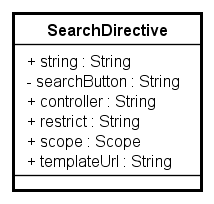
\includegraphics[scale=0.5,keepaspectratio]{UML/Classi/Front-End/QuizziPedia_Front-end_Directives_SearchDirective.png}
	\caption{QuizziPedia::Front-End::Directives::SearchDirective}
\end{figure}

\begin{itemize}
	\item \textbf{Descrizione}: directive che permette di effettuare la ricerca di utenti e questionari;
	\item \textbf{Utilizzo}: permette all'utente di effettuare ricerche, è strutturata da:
	\begin{itemize}
		\item Barra di ricerca;
		\item Pulsante per effettuare la ricerca;
	\end{itemize}
	\item \textbf{Relazioni con altre classi}:
	\begin{itemize}
			\item \textit{IN} \texttt{HomeView}: view contenente la barra di ricerca per gli utenti e questionari e il bottone che porterà l'utente nella modalità allenamento;
		\item \textit{IN} \texttt{MenuBarDirective}: rappresenta il menù, presente in ogni pagina dell'applicazione, generato in base agli oggetti passati nello \$scope isolato. Fornisce un pulsante per ogni oggetto ricevuto come parametro, ogni pulsante viene rappresentato con un’icona e con un testo. Al click di un pulsante viene invocata la funzione ad esso associata;
		\item \textit{IN} \texttt{SearchController}: questa classe permette di gestire la ricerca di questionari e utenti all'interno dell'applicazione.
	\end{itemize}
	\item \textbf{Attributi}:
	\begin{itemize}
		\item \texttt{+ controller: String}: stringa contenente il nome del controller della direttiva;
		\item \texttt{+ restict: String}: stringa che permette di definire le modalità di inserimento della direttiva all'interno della pagina;
		\item \texttt{+ scope: Scope}: oggetto scope interno della direttiva, contiene le funzionalità per gestire i dati presenti all'interno;
		\item \texttt{+ templateUrl: String}: stringa contenente il percorso del file \textit{HTML\ped{G}} che contiene la direttive.
	\end{itemize}
\end{itemize}

\paragraph{QuizziPedia::Front-End::Directives::StatisticsDirective}

\label{QuizziPedia::Front-End::Directives::StatisticsDirective}

\begin{figure}[h]
	\centering
	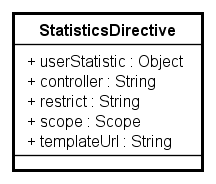
\includegraphics[scale=0.5,keepaspectratio]{UML/Classi/Front-End/QuizziPedia_Front-end_Directives_StatisticsDirective.png}
	\caption{QuizziPedia::Front-End::Directives::StatisticsDirective}
\end{figure}

\begin{itemize}
	\item \textbf{Descrizione}: directive che permette di visualizzare le statistiche di un utente;
	\item \textbf{Utilizzo}: permette di visualizzare le statistiche, in particolare viene utilizzata per mostrare statistiche:
	\begin{itemize}
		\item Nella pagina della visualizzazione del profilo;
		\item Di un utente ricercato tramite apposita funzione.
	\end{itemize}
	\item \textbf{Relazioni con altre classi}:
	\begin{itemize}
		\item \textit{IN} \texttt{UserView}: view contenente i dati personali dell'utente, le sue statistiche relative ai questionari e agli allenamenti effettuati e i questionari a cui è iscritto;
		\item \textit{IN} \texttt{OtherUserView}: view contenente i dati personali e le statistiche di un utente ricercato;
		\item \textit{IN} \texttt{StatisticsController}: questa classe permette di le statistiche di un utente;
		\item \textbf{Utilizzo}: fornisce le funzionalità per ottenere le statistiche di un utente per poterle mostrare nella view. 
	\end{itemize}
	\item \textbf{Attributi}:
	\begin{itemize}
		\item \texttt{+ controller: String}: stringa contenente il nome del controller della direttiva;
		\item \texttt{+ restict: String}: stringa che permette di definire le modalità di inserimento della direttiva all'interno della pagina;
		\item \texttt{+ scope: Scope}: oggetto scope interno della direttiva, contiene le funzionalità per gestire i dati presenti all'interno;
		\item \texttt{+ templateUrl: String}: stringa contenente il percorso del file \textit{HTML\ped{G}} che contiene la direttive.
	\end{itemize}
\end{itemize}

\paragraph{QuizziPedia::Front-End::Directives::SubscribeResultDirective }

\label{QuizziPedia::Front-End::Directives::SubscribeResultDirective}

\begin{figure}[h]
	\centering
	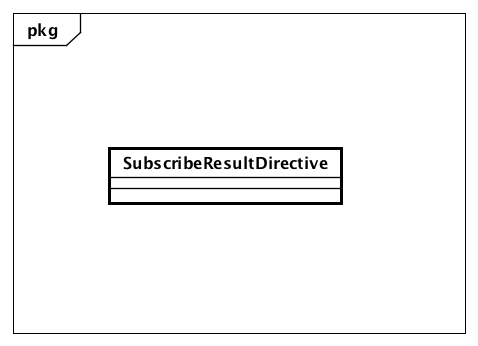
\includegraphics[scale=0.5,keepaspectratio]{UML/Classi/Front-End/QuizziPedia_Front-end_Directives_SubscribeResultDirective.png}
	\caption{QuizziPedia::Front-End::Directives::SubscribeResultDirective}
\end{figure}

\begin{itemize}
	\item \textbf{Descrizione}: directive che permette di visualizzare e iscriversi ai questionari ricercati;
	\item \textbf{Utilizzo}: permette di visualizzare e iscriversi ai questionari ricercati. Include un pulsate per ogni questionario che permette l'iscrizione ad esso.
	\item \textbf{Relazioni con altre classi}:
	\begin{itemize}
		\item \textit{IN} \texttt{ResultsView}: view contenente i risultati della ricerca effettuata, sia gli utenti che i questionari.
	\end{itemize}
	\item \textbf{Attributi}:
	\begin{itemize}
		\item \texttt{+ restict: String}: stringa che permette di definire le modalità di inserimento della direttiva all'interno della pagina;
		\item \texttt{+ scope: Scope}: oggetto scope interno della direttiva, contiene le funzionalità per gestire i dati presenti all'interno;
		\item \texttt{+ templateUrl: String}: stringa contenente il percorso del file \textit{HTML\ped{G}} che contiene la direttive.
	\end{itemize}
\end{itemize}

\paragraph{QuizziPedia::Front-End::Directives::TopicKeywordsDirective}

\label{QuizziPedia::Front-End::Directives::TopicKeywordsDirective}

\begin{figure}[h]
	\centering
	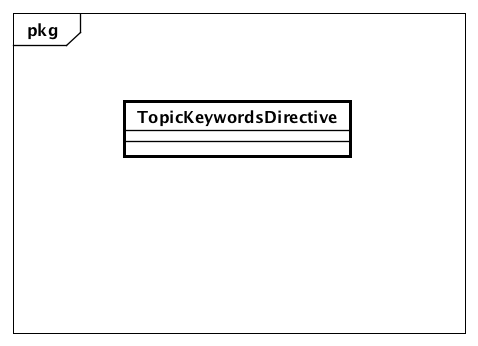
\includegraphics[scale=0.5,keepaspectratio]{UML/Classi/Front-End/QuizziPedia_Front-end_Directives_TopicKeywordsDirective.png}
	\caption{QuizziPedia::Front-End::Directives::TopicKeywordsDirective}
\end{figure}

\begin{itemize}
	\item \textbf{Descrizione}: directive che permette di gestire l'inserimento dell'argomento e delle keywords al momento della creazione della domanda;
	\item \textbf{Utilizzo}: permette l'inserimento di keywords al momento di creazione della domanda, in particolare sarà formata da:
	\begin{itemize}
		\item Un menù a tendina per selezionare l'argomento della domanda;
		\item Un campo di testo in cui inserire le keywords.
	\end{itemize}
	\item \textbf{Relazioni con altre classi}:
	\begin{itemize}
		\item \textit{IN} \texttt{CreateQuestionnaireView}: view per la creazione del questionario; 
		\item \textit{IN} \texttt{TrueFalseQuestionsView}: view contenente i campi per creare una domanda vero/falso; 
		\item \textit{IN} \texttt{MultipleQuestionsView}: view contenente i campi per creare una domanda a risposta multipla;
		\item \textit{IN} \texttt{ConnectionQuestionsView}: view contenente i campi per creare una domanda a collegamento;
		\item \textit{IN} \texttt{ImagesSortingQuestionsView}: view contenente i campi per creare una domanda a ordinamento immagini;
		\item \textit{IN} \texttt{StringsSortingQuestionsView}: view contenente i campi per creare una domanda a ordinamento stringhe;
		\item \textit{IN} \texttt{FillingQuestionsView}: view contenente i campi per creare una domanda a riempimento testo;
		\item \textit{IN} \texttt{ClickableAreaQuestionsView}: view contenente i campi per creare una domanda ad area cliccabile;
		\item \textit{IN} \texttt{EditorQMLView}: view contenente l'editor QML per la creazione di domande personalizzate;
	\end{itemize}
	\item \textbf{Attributi}:
	\begin{itemize}
		\item \texttt{+ restict: String}: stringa che permette di definire le modalità di inserimento della direttiva all'interno della pagina;
		\item \texttt{+ scope: Scope}: oggetto scope interno della direttiva, contiene le funzionalità per gestire i dati presenti all'interno;
		\item \texttt{+ templateUrl: String}: stringa contenente il percorso del file \textit{HTML\ped{G}} che contiene la direttive.
	\end{itemize}
\end{itemize}

\paragraph{QuizziPedia::Front-End::Directives::UserDetailsDirective}

\label{QuizziPedia::Front-End::Directives::UserDetailsDirective}

\begin{figure}[h]
	\centering
	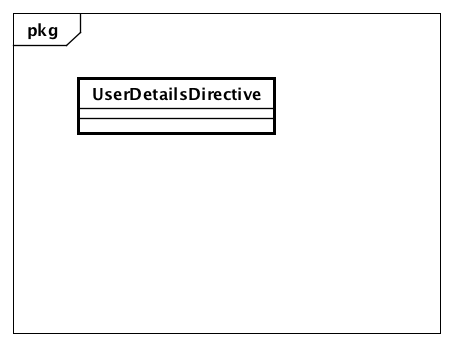
\includegraphics[scale=0.5,keepaspectratio]{UML/Classi/Front-End/QuizziPedia_Front-end_Directives_UserDetailsDirective.png}
	\caption{QuizziPedia::Front-End::Directives::UserDetailsDirective}
\end{figure}

\begin{itemize}
	\item \textbf{Descrizione}: directive che permette di visualizzare i dati personali di un utente;
	\item \textbf{Utilizzo}: permette di visualizzare i dati personali di un utente, in dettaglio conterrà:
	\begin{itemize}
		\item Nome;
		\item Cognome;
		\item Email.
	\end{itemize}
	\item \textbf{Relazioni con altre classi}:
	\begin{itemize}
		\item \textit{IN} \texttt{UserView}: view contenente i dati personali dell'utente, le sue statistiche relative ai questionari e agli allenamenti effettuati e i questionari a cui è iscritto;
		\item \textit{IN} \texttt{OtherUserView}: view contenente i dati personali e le statistiche di un utente ricercato;
		\item \textit{OUT} \texttt{UserDetailsController}: questa classe permette di gestire i dati di un utente.
	\end{itemize}
	\item \textbf{Attributi}:
	\begin{itemize}
		\item \texttt{+ controller: String}: stringa contenente il nome del controller della direttiva;
		\item \texttt{+ restict: String}: stringa che permette di definire le modalità di inserimento della direttiva all'interno della pagina;
		\item \texttt{+ scope: Scope}: oggetto scope interno della direttiva, contiene le funzionalità per gestire i dati presenti all'interno;
		\item \texttt{+ templateUrl: String}: stringa contenente il percorso del file \textit{HTML\ped{G}} che contiene la direttive.
	\end{itemize}
\end{itemize}

\paragraph{QuizziPedia::Front-End::Directives::UserResultsDirective}

\label{QuizziPedia::Front-End::Directives::UserResultsDirective}

\begin{figure}[h]
	\centering
	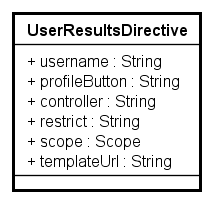
\includegraphics[scale=0.5,keepaspectratio]{UML/Classi/Front-End/QuizziPedia_Front-end_Directives_UserResultsDirective.png}
	\caption{QuizziPedia::Front-End::Directives::UserResultsDirective}
\end{figure}

\begin{itemize}
	\item \textbf{Descrizione}: directive che permette di visualizzare la lista degli utenti ricercati dopo aver utilizzato l'apposita funzione di ricerca;
	\item \textbf{Utilizzo}: permette di visualizzare la lista degli utenti, in particolare conterrà:
	\begin{itemize}
		\item Nome dell'utente;
		\item Pulsante per poter essere reindirizzati alla pagina di visualizzazione del profilo dell'utente selezionato.
	\end{itemize}
	\item \textbf{Relazioni con altre classi}:
	\begin{itemize}
		\item \textit{IN} \texttt{ResultsView}: view contenente i risultati della ricerca effettuata, sia gli utenti che i questionari.
	\end{itemize}
	\item \textbf{Attributi}:
	\begin{itemize}
		\item \texttt{+ restict: String}: stringa che permette di definire le modalità di inserimento della direttiva all'interno della pagina;
		\item \texttt{+ scope: Scope}: oggetto scope interno della direttiva, contiene le funzionalità per gestire i dati presenti all'interno;
		\item \texttt{+ templateUrl: String}: stringa contenente il percorso del file \textit{HTML\ped{G}} che contiene la direttive.
	\end{itemize}
\end{itemize}
